\documentclass[11pt]{article}

\usepackage[a4paper,margin=25mm,headheight=14pt]{geometry}
\usepackage[T1]{fontenc}
\usepackage[utf8]{inputenc}
\usepackage{lmodern}
\usepackage{microtype}
\usepackage{booktabs}
\usepackage{longtable}
\usepackage{tabularx}
\usepackage{array}
\usepackage{pdflscape}
\usepackage{graphicx}
\usepackage{xcolor}
\usepackage{caption}
\usepackage{enumitem}
\usepackage{natbib}
\usepackage{placeins}
\usepackage[hidelinks]{hyperref}

\definecolor{draftred}{HTML}{9B2C2C}
\newcommand{\verify}[1]{\textcolor{draftred}{[\textbf{#1}]}}
\newcommand{\authorconfirm}[1]{\textcolor{draftred}{[\textbf{#1}]}}
\newcommand{\journalverify}[1]{\textcolor{draftred}{[\textbf{#1}]}}
\newcommand{\aiverify}[1]{\textcolor{draftred}{[\textbf{#1}]}}
% Internal workflow state is retained in source and QA, but is intentionally
% suppressed from the professor-facing PDF. The factual ethics sentence remains visible.
\newcommand{\ethicspending}[1]{}
\newcolumntype{P}[1]{>{\raggedright\arraybackslash}p{#1}}

\title{\textbf{Reproducibility and Data Quality of Bangladesh's Public DGHS Dengue Dashboard: An Empirical Evaluation}}
\author{Tajrian Sarwar \textperiodcentered\ Md Aminul Islam}
\date{}

\begin{document}
\maketitle

\begin{abstract}
\noindent\textbf{Background:}

Public dengue dashboards can support timely secondary research, but a visible value is not necessarily a documented, semantically stable, or reproducible research observation. We evaluated the public Bangladesh Directorate General of Health Services (DGHS) Dengue Dynamic Dashboard as a research-data interface.

The objective was to assess historical-state reproducibility, provenance, semantic interpretability, and internal reconciliation while preserving the boundary between dashboard observations and the underlying surveillance system.

\medskip\noindent\textbf{Methods:}

We reconstructed validated historical dashboard states from 2024--2026 using a provenance-preserving workflow. Exact responses were archived with SHA-256 integrity hashes, then assessed using source labels, semantic contracts, reconciliation checks, and a bounded revision/stability audit. Analysis remained descriptive and restricted to dashboard-reported observations.

\medskip\noindent\textbf{Results:}

The 27 validated historical states spanning 2024--2026 were successfully reconstructed with traceable response, date, and integrity records. The returned content exposed concrete category anomalies, including overlapping age bands, malformed or numeric-looking labels, spelling variants, and geographically ambiguous source labels. Reconciliation was restricted where reporting windows, semantic universes, or typed longitudinal values were incompatible or unavailable. Retrospective revision/stability remained unresolved because repeated typed chart-point values were unavailable. The 2026 states were incomplete and were not treated as a completed annual period (Supplementary Table S1).

\medskip\noindent\textbf{Conclusions:}

The dashboard supported traceable reconstruction of selected historical states and bounded use of source-labelled observations, but retrieval did not resolve case semantics, reporting-facility coverage, geographic attribution, denominator compatibility, or revision behavior. Secondary users should archive raw responses, preserve labels, validate semantic compatibility, and distinguish dashboard observations from the underlying surveillance system.

\end{abstract}

\section{Introduction}
Dengue surveillance in Bangladesh operates at the intersection of a recurrent public-health problem and a reporting system that must support rapid operational decisions. The country's dengue evidence base includes hospital and clinical reporting, outbreak communications, spatial analyses, and predictive work, while the national surveillance architecture remains dependent on the quality, timeliness, and interpretability of the observations that reach public reporting interfaces \citep{ref1,ref6}. This distinction matters because a value that is publicly visible is not automatically equivalent to a complete measure of infection, a population denominator, or a stable representation of the underlying surveillance system.

Recent literature demonstrates substantial analytic activity using Bangladesh dengue observations. National analyses have examined temporal and geographic patterns across 2019--2023 \citep{ref2}, and district-level hotspot and cluster methods have been applied to the 2023 outbreak \citep{ref3}. A 2026 retrospective ecological study extends this broad precedent across all 64 districts using reported hospital admissions \citep{ref4}. These studies establish that national, district, and spatial dengue analyses are already represented in the literature. They also make the provenance and interpretation of shared surveillance observations consequential: the scientific question is not only what a dashboard value appears to show, but also which reporting universe, time window, geography, and revision state it represents.

System-level assessments provide an important reason to examine these properties explicitly. A recent narrative review describes Bangladesh's dengue surveillance as involving passive and active modalities, with passive and hospital-based reporting offering wide coverage but remaining vulnerable to underreporting and delayed notification \citep{ref1}. The same review identifies variability in data quality, timeliness, interoperability, and terminology, and notes limited standardization in the explicit reporting of case or outbreak definitions \citep{ref1}. The World Health Organization's Bangladesh country assessment likewise treats communicable-disease surveillance as an architecture requiring mapping, performance evaluation, and opportunities for integration and improvement, with dengue included among the priority diseases considered \citep{ref6}. An official 2023 situation report further describes hospital-based surveillance, regular information from hospitals and Upazila and district facilities, and daily dissemination through the Health Emergency Operations Center \citep{ref7}. Together, these sources support a layered interpretation: public dashboard observations are outputs of a surveillance and reporting environment, not transparent substitutes for that environment.

The public DGHS Dengue Dynamic Dashboard is therefore an important research-data interface. Its accessibility can support reproducible observation of historical dashboard states, but accessibility alone does not establish that a response can be reconstructed, that displayed fields are semantically interchangeable, or that geographic labels identify patient residence rather than a facility or administrative reporting universe. A publicly available non-peer-reviewed reproducible analysis repository already describes a national analysis based on DGHS HEOC dashboard-derived aggregate surveillance data \citep{ref5}. That repository is relevant grey-literature prior art and further prohibits framing reproducibility of DGHS-derived dengue data as a first-in-field contribution. Its presence also reinforces the need to state precisely what a new study audits: the source interface, its exposed observations, and the evidentiary limits surrounding their interpretation.

ResearchDengu addresses this narrower methodological problem. The study evaluates whether selected historical states of the public DGHS dashboard can be reconstructed and preserved as research artifacts, and whether their source-labelled fields can be interpreted without silently converting them into population-level measures. The primary object is the dashboard as a public surveillance-data interface rather than Bangladesh dengue burden, transmission, climate association, spatial risk, or prediction. Restricted descriptive dengue observations are retained to show the structure and use of the interface, but they are not used to estimate incidence, prevalence, risk, causal effects, or the completeness of the national surveillance system.

The study has four linked aims. First, it documents the provenance of archived dashboard responses through date-specific acquisition records and cryptographic hashes. Second, it evaluates whether the observed HTML, chart, control, and table structures support reproducible reconstruction of selected dashboard states. Third, it preserves raw labels and tests semantic questions that affect comparability, including reporting windows, category definitions, and geographic meaning. Fourth, it records internal reconciliation limitations and unresolved revision or stability questions without correcting, imputing, or biologically interpreting them. The resulting contribution is consequently a provenance-preserving observation-level reproducibility and data-quality audit.

This framing is deliberately bounded by the existing literature. ResearchDengu does not claim to be the first nationwide dengue analysis, the first reproducible Bangladesh dengue dataset, or the first surveillance-quality study in Bangladesh \citep{ref1,ref2,ref3,ref4,ref5,ref6,ref7}. Instead, it complements national and district epidemiological studies by making the data-interface layer inspectable: what was requested, what was returned, what was displayed, how it was archived, and which claims remain unsupported. The Methods and Results that follow therefore distinguish dashboard-level reproducibility from underlying surveillance validity and describe all retained values using the source terminology and limitations recorded in the project's evidence contracts.

\section{Methods}
\subsection{Study design}

We conducted an observation-level surveillance-methods and data-quality study of historical states exposed by the public Directorate General of Health Services (DGHS) Dengue Dynamic Dashboard. Restricted descriptive dengue observations were retained as supporting context. The study was designed to assess reproducibility, semantic interpretability, provenance, and internal reconciliation rather than to estimate population disease burden or causal effects.

\subsection{Data source and DGHS Dengue Dynamic Dashboard}

The data source was the publicly accessible DGHS Dengue Dynamic Dashboard. The study used dashboard responses archived during the project's validated acquisition process. Public-dashboard observations were not assumed to constitute the underlying DGHS surveillance database. The available source fields were therefore described using source terminology and were not reinterpreted as population-level measures.

The validated corpus comprised 27 dated snapshots from 1 January 2024 through 29 September 2026 (Supplementary Table S1). The 2026 observations were treated as an incomplete follow-up period and were not treated as a completed annual observation.

\subsection{Historical dashboard-state reconstruction}

For this study, a historical dashboard state was considered successfully reconstructed when the validated acquisition record showed that the requested date and year were submitted, the public response returned HTTP 200, a displayed dashboard date was extracted and agreed with the requested date, the expected dashboard structure was present, and the required source-labelled fields could be extracted. The raw response was archived before parsing, request/response metadata were recorded, and a SHA-256 integrity hash was calculated. Expected structure was checked with a deterministic compatibility signature: a SHA-256 hash of normalized JSON containing every form's method, normalized action, and control tuples (element name, type, name); all table-header text lists; and the sorted IDs of the specified chart containers. The reference signature was \texttt{84efb756f47cbb24e1ad240bc2507576ead9cab3951e379ac0e618e7bb94a83d}. This is structural compatibility only and does not establish semantic equivalence. The frozen ledger records these criteria for all 27 states; the three B1.7 spot-validated states additionally passed all 18 offline source-to-table checks (Supplementary Tables S1--S2).

\subsection{Acquisition protocol and sampling}

The acquisition workflow used ordinary public requests to the dashboard's documented interface, without authentication, CAPTCHA circumvention, access-control bypass, endpoint guessing, or browser automation. The exact response body was archived before parsing under date-specific directories with metadata and SHA-256 integrity hashes. The 27-date set contains 9 dates in each of 2024, 2025, and 2026. The 2024--2025 dates were predefined candidates retained from the B0.9A/B0.9C manifest, including year and month boundaries, selected dated states, and year-validation dates. The 2026 dates were predefined validated B0.8A/B pilot dates. The ledger records 16 retrieved-valid and 11 reused-verified artifacts, with no acquisition failure substitution. The available manifests do not preserve a complete chronology of whether any candidate was viewed before final selection; accordingly, the study does not claim an outcome-blinded sampling process. Full date-level bases and statuses are provided in Supplementary Table S3.

\subsection{Archived response integrity and provenance}

Each archived response was retained as a project artifact and identified by a SHA-256 integrity digest. Hashing supports later integrity verification; it does not by itself establish write-once storage or retention control. The B0.10 freeze linked processed observations and headline tables to parent responses. The B0.11 and B1.7 manifests were checked before drafting, and the frozen B0.10 processed-table hashes remained unchanged. Provenance completeness was assessed across 432 processed observations (Supplementary Table S1).

\subsection{Data extraction}

Extraction retained objectively present HTML tables, chart or script-derived source labels, controls, and headline fields. The processed observation table represented 11 data families across the 27 snapshots, yielding 297 family-level observation rows. The authorized headline-derived table retained four source-labelled fields per snapshot---weekly case, weekly death, cumulative case, and cumulative death---corresponding to 108 field values across the corpus (Supplementary Table S1).

The B1.7 spot-validation confirmed that these headline values were represented in the dashboard summary strip using the weekly and cumulative icon fields. The separate last-24-hour charts were treated as a different reporting window and were not substituted for the summary-strip fields (Supplementary Table S1).

\subsection{Semantic validation}

Semantic validation followed the B0.11 variable, language, age-label, and geography contracts. Values were described as DGHS-reported dashboard observations or source-labelled fields. The dashboard response was not treated as evidence of patient residence, treatment location, reporting-facility coverage, population denominators, infection status, or underlying surveillance-system validity.

\subsection{Category normalization}

Normalization was conservative and provenance-preserving. Raw labels were retained. Blank, malformed, overlapping, spacing-variant, and otherwise ambiguous categories were not silently repaired, merged, redistributed, or imputed. Source \texttt{Male} and \texttt{Female} labels were retained as sex-labelled dashboard categories; no gender identity or broader sex concept was inferred. Geography labels, including \texttt{Out of CC}, were not converted into residence or population categories.

\subsection{Internal reconciliation procedures}

Existing B0.10 reconciliation checks were retained without correction. The audit contained nine reconciliation tests, including demographic, geographic, headline, and longitudinal compatibility checks. B0.11 classified nine reconciliation limitations according to differences in time window, missing or unclassified categories, semantic mismatch, and unresolved compatibility. These classifications describe evidence limitations; they do not establish causal surveillance-system failures.

\subsection{Historical revision/stability assessment}

Revision assessment used the frozen B0.11 revision audit. Four time-unit rows---daily, EPI-week, monthly, and annual---remained unresolved because the processed parent did not contain typed chart-point values sufficient to construct canonical repeated series. Accordingly, the study did not claim that the dashboard was stable or that a revision process had been established.

\subsection{Restricted descriptive analysis}

Descriptive analysis was limited to source-labelled snapshot fields, family availability, anomaly counts, reconciliation classifications, provenance completeness, and bounded descriptive observations. No rates, incidence estimates, prevalence estimates, risk estimates, forecasts, regression, hypothesis tests, inferential confidence intervals, spatial inference, or causal analyses were performed. The 2026 period was explicitly treated as incomplete.

\subsection{Reproducibility verification}

Results were verified against the frozen B1 provenance records and B1.7 paper-package artifacts. Seven core findings were independently validated. In addition, three archived snapshots---2024-01-01, 2025-09-29, and 2026-09-29---were checked against the summary-strip labels, headline values, date controls, and displayed dates; all 18 checks matched (Supplementary Table S1).

\subsection{Ethics and data governance}

The study used publicly accessible aggregate dashboard observations and the project's archived responses. No patient-level identifiers were processed in the analyzed tables. Formal institutional review or exemption status has not yet been determined.


\begin{figure}[htbp]
\centering
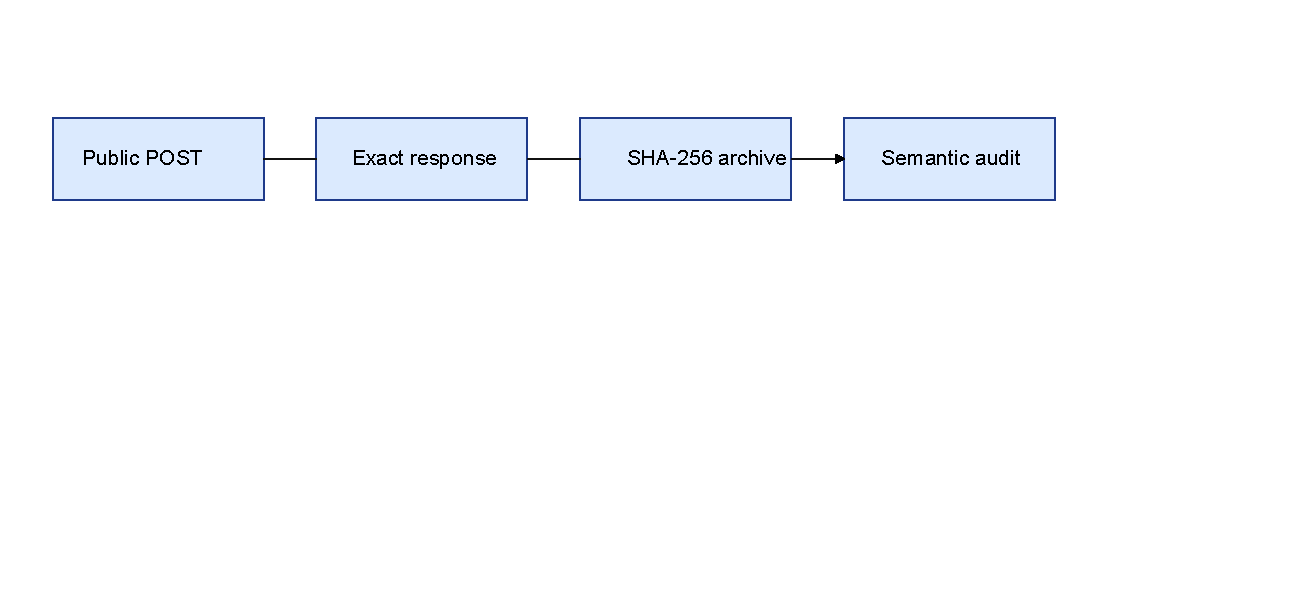
\includegraphics[width=0.92\linewidth]{figures/figure1_acquisition_workflow.pdf}
\caption{Validated acquisition workflow for historical dashboard-state reconstruction.}
\label{fig:acquisition-workflow}
\caption*{\footnotesize Source: ResearchDengu B0.10/B1 frozen dashboard artifacts; 2024--2026 snapshots. Limitation: source-labelled dashboard observations; not population incidence, risk, or causal evidence.}
\end{figure}
\FloatBarrier

\section{Results}
\subsection{Dataset and snapshot sampling}

The analysis-ready corpus contained 27 dated dashboard snapshots spanning 1 January 2024 to 29 September 2026. There were 9 dates in each year. The 2024--2025 dates were manifest-defined candidates retained from the B0.9A/B0.9C range design, with year boundaries, month boundaries, selected dated states, and year-validation dates. The 2026 dates were the validated B0.8A/B pilot set. All 27 manifest rows were represented in the historical ledger; 16 were recorded as retrieved-valid and 11 as reused-verified artifacts, with no documented acquisition failure substitution. The available records do not establish whether every selection decision preceded viewing all possible outcomes, so the sample is described as predefined in the manifest, not as outcome-blinded or representative (Supplementary Table S3).

This design supplies an auditable set of historical states rather than a claim of continuous daily coverage. It also distinguishes newly retrieved responses from previously verified artifacts, which is relevant when a later user attempts to reproduce the archive or interpret differences between dates.

\subsection{Operational reconstruction and provenance}

All 27 archived states had recorded submitted dates, HTTP 200 responses, displayed dates matching the requested dates, the reference structural compatibility signature (\texttt{84efb756f47cbb24e1ad240bc2507576ead9cab3951e379ac0e618e7bb94a83d}), response metadata, and SHA-256 records. The signature summarizes normalized form structure, table headers, and selected chart-container IDs; it is not a semantic claim. The frozen processed outputs represented 11 data families across the 27 snapshots, yielding 297 family-level rows. Four source-labelled headline fields were retained per snapshot, yielding 108 field values. All 432 processed observations retained provenance fields. For the three B1.7 spot-validated snapshots---2024-01-01, 2025-09-29, and 2026-09-29---18 checks of date controls, displayed dates, summary-strip labels, and headline values all matched. These checks demonstrate reproducible reconstruction within the archived corpus; they do not demonstrate complete upstream surveillance coverage (Supplementary Tables S1--S3).

\subsection{Semantic and category findings}

The 11-row anomaly register shows concrete examples of why raw-label preservation was necessary. In the age-by-sex family, \texttt{0-10} overlaps with \texttt{0-5} and \texttt{6-10}; \texttt{06-10} and \texttt{6-10} are format variants that were not shown to be safely mergeable; and \texttt{42309} and \texttt{46301} are numeric-looking labels without an established age meaning. In the division family, \texttt{Raishahi} was preserved separately from \texttt{Rajshahi} rather than silently corrected. Geographic examples included \texttt{Dhaka Division (Out of CC)}, whose residence/facility/administrative meaning remained unresolved, and the raw \texttt{DNCC} and \texttt{DSCC} City Corporation labels. These labels were not converted into rural, urban-population, or patient-residence categories. Age-by-sex and death-age-by-sex families were unavailable in the frozen processed table for all 27 snapshots. The complete register and treatment decisions are in Table-Category-Anomalies and the B0.11 semantic maps.

\subsection{Internal reconciliation findings}

The nine reconciliation tests show different forms of restricted comparability. The weekly-case versus cumulative-case comparison was retained as a non-identity audit comparison, not an arithmetic equality. Age-by-sex component tests remained unresolved because raw labels and table-to-family universes were not frozen. Within/outside City Corporation and division subtotal comparisons were not comparable because geographic attribution and compatible denominators were not established. Daily, EPI-week, and monthly accumulation tests remained unresolved because typed series and compatible totals were unavailable. Weekly and cumulative death quantities were not summed because they represent different reporting windows. The B0.11 classifications therefore identify missing categories, semantic mismatch, different time windows, unknown compatibility, or dashboard-raw reconciliation limitations; they do not call these observations biological or system failures (Table-Reconciliation-Audit).

\subsection{Revision and stability findings}

The revision audit contains four entries---daily, EPI-week, monthly, and annual---and each is \texttt{UNRESOLVED}. The frozen processed parent contains family-level observations but not typed repeated chart-point values linked to a stable observation identity across captures. Establishing retrospective revision would have required repeated typed values for the same historical point, with stable time keys and comparable field definitions. Because that evidence was absent, the study did not demonstrate that revisions occurred, that the dashboard was stable, or that a revision policy existed (Table-Revision-Stability-Audit).

\subsection{Restricted descriptive observations}

The three predefined illustrative snapshots make the source-labelled headline structure visible. On 2024-01-01, the weekly and cumulative case fields were both 82 and the corresponding death fields were both 0. On 2025-09-29, the weekly case and death fields were 1,579 and 7, while cumulative case and death fields were 46,783 and 195. On 2026-09-29, the corresponding values were 6,136 and 20, and 77,672 and 239. Equality of weekly and cumulative values in an individual snapshot does not establish semantic equivalence between the fields. All three snapshots passed the 18-check B1.7 spot-validation. These are source-labelled dashboard fields, not population incidence, risk, or community infection estimates; 2026 remains incomplete (Table-Illustrative-Headline-Snapshots).


\subsection*{Table 1. DGHS dashboard data families and semantic/readiness status}
\begingroup\footnotesize\setlength{\tabcolsep}{3pt}\renewcommand{\arraystretch}{1.15}
\begin{longtable}{P{0.1920\linewidth}P{0.1920\linewidth}P{0.1920\linewidth}P{0.1920\linewidth}P{0.1920\linewidth}}
\toprule
Data family & Snapshots & Present & Not available & Semantic status \\
\midrule\endhead
age\_by\_sex & 27 & 0 & 27 & RESTRICTED\_SOURCE\_LABEL\_ONLY \\
annual\_series & 27 & 27 & 0 & RESTRICTED\_SOURCE\_LABEL\_ONLY \\
city\_corporation\_data & 27 & 27 & 0 & RESTRICTED\_SOURCE\_LABEL\_ONLY \\
daily\_series & 27 & 27 & 0 & RESTRICTED\_SOURCE\_LABEL\_ONLY \\
death\_age\_by\_sex & 27 & 0 & 27 & RESTRICTED\_SOURCE\_LABEL\_ONLY \\
division\_by\_epi\_week & 27 & 27 & 0 & RESTRICTED\_SOURCE\_LABEL\_ONLY \\
division\_data & 27 & 27 & 0 & RESTRICTED\_SOURCE\_LABEL\_ONLY \\
epi\_week\_series & 27 & 27 & 0 & RESTRICTED\_SOURCE\_LABEL\_ONLY \\
headline\_metrics & 27 & 27 & 0 & RESTRICTED\_SOURCE\_LABEL\_ONLY \\
monthly\_series & 27 & 27 & 0 & RESTRICTED\_SOURCE\_LABEL\_ONLY \\
within\_outside\_city\_corporation & 27 & 0 & 27 & RESTRICTED\_SOURCE\_LABEL\_ONLY \\
\bottomrule
\end{longtable}
\endgroup

\noindent\emph{Family presence is not semantic comparability.}

\begin{landscape}
\subsection*{Table 2. Historical snapshot and reproducibility characteristics}
\begingroup\footnotesize\setlength{\tabcolsep}{3pt}\renewcommand{\arraystretch}{1.15}
\begin{longtable}{P{0.1600\linewidth}P{0.1600\linewidth}P{0.1600\linewidth}P{0.1600\linewidth}P{0.1600\linewidth}P{0.1600\linewidth}}
\toprule
Snapshot & Year & Requested date & Displayed date & Headline observations & Semantic status \\
\midrule\endhead
2024-01-01 & 2024 & 2024-01-01 & 2024-01-01 & 4 & SUPPORTED\_MEANING \\
2024-01-31 & 2024 & 2024-01-31 & 2024-01-31 & 4 & SUPPORTED\_MEANING \\
2024-02-01 & 2024 & 2024-02-01 & 2024-02-01 & 4 & SUPPORTED\_MEANING \\
2024-02-28 & 2024 & 2024-02-28 & 2024-02-28 & 4 & SUPPORTED\_MEANING \\
2024-03-01 & 2024 & 2024-03-01 & 2024-03-01 & 4 & SUPPORTED\_MEANING \\
2024-04-04 & 2024 & 2024-04-04 & 2024-04-04 & 4 & SUPPORTED\_MEANING \\
2024-04-30 & 2024 & 2024-04-30 & 2024-04-30 & 4 & SUPPORTED\_MEANING \\
2024-06-30 & 2024 & 2024-06-30 & 2024-06-30 & 4 & SUPPORTED\_MEANING \\
2024-09-29 & 2024 & 2024-09-29 & 2024-09-29 & 4 & SUPPORTED\_MEANING \\
2025-01-01 & 2025 & 2025-01-01 & 2025-01-01 & 4 & SUPPORTED\_MEANING \\
2025-01-31 & 2025 & 2025-01-31 & 2025-01-31 & 4 & SUPPORTED\_MEANING \\
2025-02-01 & 2025 & 2025-02-01 & 2025-02-01 & 4 & SUPPORTED\_MEANING \\
2025-02-28 & 2025 & 2025-02-28 & 2025-02-28 & 4 & SUPPORTED\_MEANING \\
2025-03-01 & 2025 & 2025-03-01 & 2025-03-01 & 4 & SUPPORTED\_MEANING \\
2025-04-04 & 2025 & 2025-04-04 & 2025-04-04 & 4 & SUPPORTED\_MEANING \\
2025-04-30 & 2025 & 2025-04-30 & 2025-04-30 & 4 & SUPPORTED\_MEANING \\
2025-06-30 & 2025 & 2025-06-30 & 2025-06-30 & 4 & SUPPORTED\_MEANING \\
2025-09-29 & 2025 & 2025-09-29 & 2025-09-29 & 4 & SUPPORTED\_MEANING \\
2026-01-01 & 2026 & 2026-01-01 & 2026-01-01 & 4 & SUPPORTED\_MEANING \\
2026-01-31 & 2026 & 2026-01-31 & 2026-01-31 & 4 & SUPPORTED\_MEANING \\
2026-02-01 & 2026 & 2026-02-01 & 2026-02-01 & 4 & SUPPORTED\_MEANING \\
2026-02-28 & 2026 & 2026-02-28 & 2026-02-28 & 4 & SUPPORTED\_MEANING \\
2026-03-01 & 2026 & 2026-03-01 & 2026-03-01 & 4 & SUPPORTED\_MEANING \\
2026-04-04 & 2026 & 2026-04-04 & 2026-04-04 & 4 & SUPPORTED\_MEANING \\
2026-04-30 & 2026 & 2026-04-30 & 2026-04-30 & 4 & SUPPORTED\_MEANING \\
2026-06-30 & 2026 & 2026-06-30 & 2026-06-30 & 4 & SUPPORTED\_MEANING \\
2026-09-29 & 2026 & 2026-09-29 & 2026-09-29 & 4 & SUPPORTED\_MEANING \\
\bottomrule
\end{longtable}
\endgroup

\noindent\emph{Provenance completeness does not resolve meaning.}
\end{landscape}

\subsection*{Table 3. Data-quality anomalies and reconciliation findings}
\begingroup\footnotesize\setlength{\tabcolsep}{3pt}\renewcommand{\arraystretch}{1.15}
\begin{longtable}{P{0.1920\linewidth}P{0.1920\linewidth}P{0.1920\linewidth}P{0.1920\linewidth}P{0.1920\linewidth}}
\toprule
Result ID & Metric & Value & Classification & Limitation \\
\midrule\endhead
B1-Q-001 & B0.10 anomaly rows & 11 & SEMANTIC UNCERTAINTY & Descriptive audit count; not an epidemiological estimate \\
B1-Q-002 & B0.10 reconciliation rows & 9 & SEMANTIC UNCERTAINTY & Descriptive audit count; not an epidemiological estimate \\
B1-Q-003 & B0.11 revision audit unresolved rows & 4 & SEMANTIC UNCERTAINTY & Descriptive audit count; not an epidemiological estimate \\
B1-Q-004 & B0.11 classified reconciliation failures & 9 & SEMANTIC UNCERTAINTY & Descriptive audit count; not an epidemiological estimate \\
B1-Q-005 & B0.10 processed rows with provenance fields & 432 & SOURCE/DASHBOARD OBSERVATION & Descriptive audit count; not an epidemiological estimate \\
\bottomrule
\end{longtable}
\endgroup

\noindent\emph{Counts are audit categories, not causal system-failure estimates.}

\begin{table}[htbp]
\centering
\caption{Illustrative source-labelled headline snapshots.}
\label{tab:headline-snapshots}
\small
\begin{tabularx}{\linewidth}{@{}lrrrr@{}}
\toprule
Displayed date & Weekly case & Weekly death & Cumulative case & Cumulative death \\
\midrule
2024-01-01 & 82 & 0 & 82 & 0 \\
2025-09-29 & 1,579 & 7 & 46,783 & 195 \\
2026-09-29 & 6,136 & 20 & 77,672 & 239 \\
\bottomrule
\end{tabularx}
\caption*{Source-labelled dashboard fields; 2026 remains incomplete. Equality of weekly and cumulative values in an individual snapshot does not establish semantic equivalence between the fields.}
\end{table}

\begin{figure}[htbp]
\centering
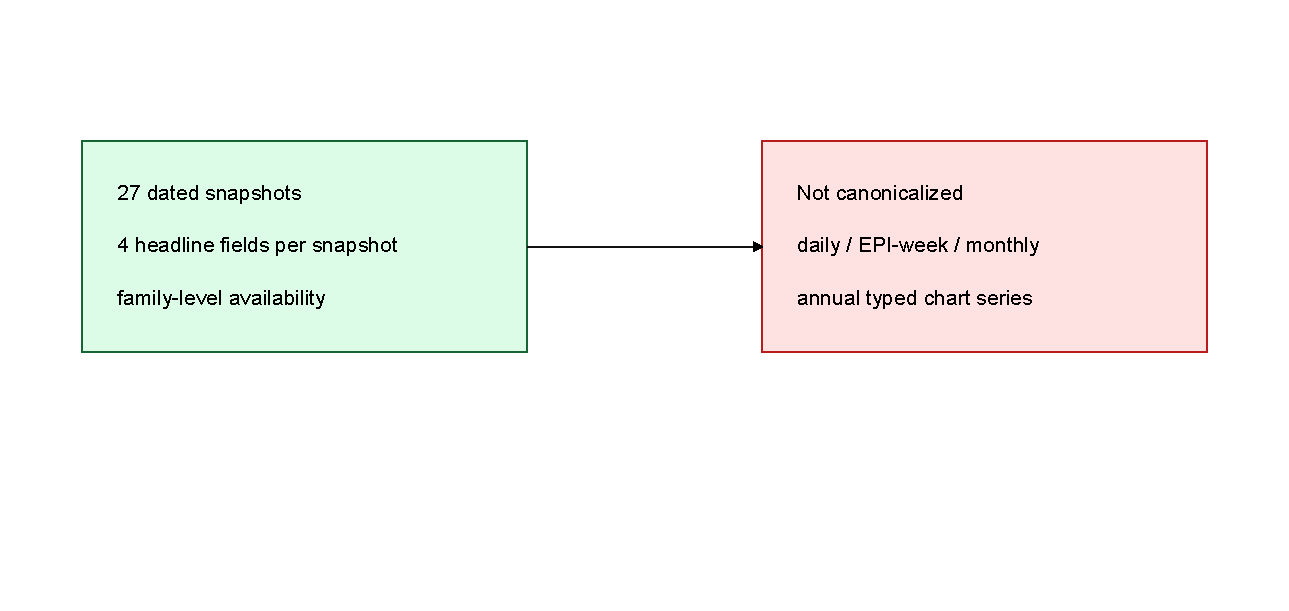
\includegraphics[width=0.92\linewidth]{figures/figure2_snapshot_structure.pdf}
\caption{Historical snapshot-level reconstruction and unavailable longitudinal structure. The 2026 period is incomplete, and dashboard responses are not treated as the underlying database.}
\label{fig:snapshot-structure}
\caption*{\footnotesize Source: ResearchDengu B0.10/B1 frozen dashboard artifacts; 2024--2026 snapshots. Limitation: snapshot-level values are reproducible within the frozen archive; typed longitudinal chart values remain unavailable.}
\end{figure}

\begin{figure}[htbp]
\centering
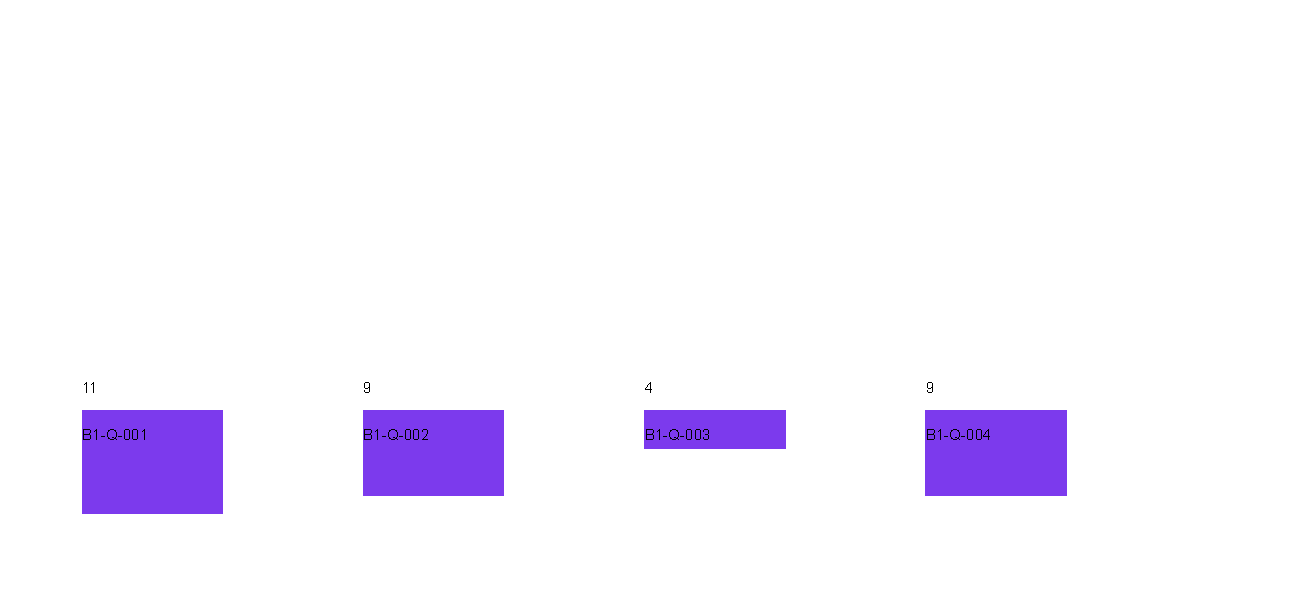
\includegraphics[width=0.92\linewidth]{figures/figure3_quality_findings.pdf}
\caption{Surveillance-quality anomalies and reconciliation findings. Counts are audit categories and are not interpreted as causal system-failure estimates.}
\label{fig:quality-findings}
\caption*{\footnotesize Source: ResearchDengu B0.10/B1 frozen dashboard artifacts; 2024--2026 snapshots. Limitation: counts are audit categories, not causal system-failure estimates.}
\end{figure}

\begin{figure}[htbp]
\centering
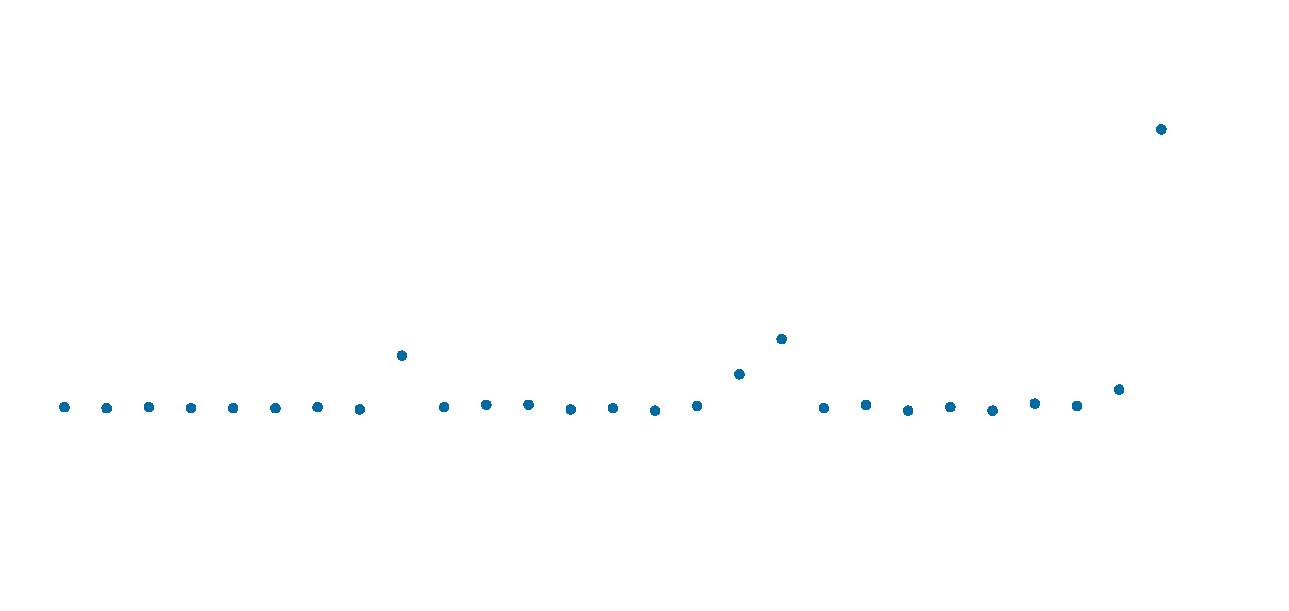
\includegraphics[width=0.92\linewidth]{figures/figure4_restricted_headline_observations.pdf}
\caption{Restricted source-labelled headline observations. Snapshot points are not an inferential trend, and 2026 is incomplete.}
\label{fig:headline-observations}
\caption*{\footnotesize Source: ResearchDengu B0.10/B1 frozen dashboard artifacts; 2024--2026 snapshots. Limitation: source-labelled observations are not population incidence, risk, or causal evidence; 2026 is incomplete and is not a completed-year comparison.}
\end{figure}

\FloatBarrier

\section{Discussion}
\subsection{Principal findings}

The audit demonstrates that the public DGHS Dengue Dynamic Dashboard can serve as a bounded research-data interface when the requested state, returned response, displayed date, extracted fields, and integrity record are documented together. This is a reproducibility result for the frozen archive, not evidence that all dashboard history or all upstream reporting was captured. The empirical tables show why this distinction matters: raw labels, compatible universes, and typed longitudinal values cannot be assumed from visual availability alone.

The most consequential interpretation is that provenance and semantics are complementary. A response can be archived and hash-checked while its age category, geography, admission terminology, or reporting window remains incompletely defined. The study therefore makes an observation-to-table path inspectable without treating traceability as proof of population meaning. Source-labelled headline observations remain usable for restricted description, while normalized demographic or geographic comparisons remain limited by the contracts documented in B0.11.

\subsection{Relationship to existing Bangladesh dengue research}

Bangladesh already has national temporal and geographic analyses, district hotspot work, broad 64-district ecological analysis, surveillance-system assessment, and hospital/passive reporting literature \citep{ref1,ref2,ref3,ref4,ref6,ref7}. A publicly available non-peer-reviewed reproducible analysis repository also describes a DGHS HEOC dashboard-derived national analysis \citep{ref5}. ResearchDengu therefore does not add another burden, spatial, climate, predictive, or transmission analysis. It examines a different layer: the publicly exposed dashboard state as a research interface requiring provenance, semantic interpretation, and internal-consistency checks.

This distinction is substantive. Prior studies can use reported observations to answer epidemiological questions, while a dashboard audit asks whether a secondary researcher can reconstruct and interpret the exposed observation without silently changing its universe. An unresolved dashboard-level semantic issue does not establish a defect in the complete DGHS surveillance system, just as reproducible retrieval does not establish a complete national account. The present study complements, rather than replaces, epidemiological and system-level work.

The distinction also affects how apparent agreement should be read. A matching number across two panels may reflect shared display logic, but it does not demonstrate that the panels describe the same reporting population or time window. Conversely, a mismatch may be expected when one field is weekly and another cumulative, or when a geographic chart uses a different administrative universe. The reconciliation table therefore adds interpretive information even where it does not produce a corrected value: it tells a future user which comparisons are defensible and which should remain open.

\subsection{Implications for epidemiological researchers}

Acquisition should be treated as part of measurement documentation. Researchers should record the public submission, retrieval time, requested and displayed dates, response status, returned structure, raw response, and SHA-256 integrity hash before parsing. They should preserve source terminology and distinguish weekly, cumulative, daily, EPI-week, monthly, and annual fields until compatible definitions are established. A label that appears in a chart is not self-interpreting if its numerator, denominator, reporting pathway, or geographic assignment is undocumented.

Reconciliation should be attempted only after the compared fields are shown to share a reporting universe and time window. An unresolved or not-comparable result is preferable to forced totals, imputation, or a claim of system failure. Repeated captures are also required before a changed historical state can be characterized as a revision pattern. These practices allow researchers to use bounded dashboard observations without converting them into patient-residence, population, or community measures.

The sampling record has a related implication. Calendar anchors and pilot dates can make a corpus auditable, but they do not make it representative of every day or every reporting transition. Users should distinguish a predefined archive from a complete surveillance time series and should report whether a state was newly retrieved or reused from an earlier verified artifact. That distinction is especially important when a later analysis compares apparent changes across years or attempts to reproduce a historical display.

\subsection{Implications for public surveillance-data publication}

The findings suggest publication principles that could improve secondary use without imposing an obligation on DGHS. Stable metadata should identify case or admission definitions, reporting universe, time window, geographic meaning, and the relation between interval and cumulative fields. Machine-readable historical exports should retain release or retrieval dates, data dictionaries, stable field names, and version or change information. Geographic fields would be more interpretable with stable administrative codes and an explicit distinction between residence, treatment facility, reporting facility, and administrative aggregation. These are design recommendations, not claims that the current dashboard must implement them.

For secondary users, these principles would make an important distinction visible at the point of download: whether a value is a source observation, an updated version of a previous observation, or an analyst-derived summary. A documented change history would also allow a researcher to cite the state actually used rather than relying only on the date displayed in a browser. Clear labels for unavailable families and unresolved definitions would reduce pressure to fill gaps through ad hoc normalization. None of these recommendations changes the evidentiary status of the current corpus; they describe information that would make future public data states easier to reproduce and interpret.

\subsection{Strengths}

Strengths include a predefined acquisition/validation scope, archived response bodies with SHA-256 integrity hashes, raw-label preservation, semantic contracts, explicit reconciliation classifications, result-level provenance, independent numerical verification, and manual spot-validation. The study also separates restricted descriptive reporting from unsupported epidemiological inference. These features support auditability of the project corpus but do not remove the limitations below.

\subsection{Limitations}

The study evaluates publicly exposed dashboard states, not the complete underlying DGHS surveillance database. The dashboard may reflect hospital or passive surveillance; retrieval does not measure community ascertainment, health-seeking behavior, notification completeness, or all upstream records. Case, admission, and death semantics remain incompletely documented, and reporting-facility coverage may vary across dates. Geographic attribution is unresolved: district and City Corporation labels were not established as residence, treatment location, reporting facility, or another administrative unit.

Population denominators and numerator compatibility were not established, so the study does not estimate population incidence, prevalence, or individual risk. Historical coverage is limited to the validated snapshots and cadence points; 2026 is incomplete and is not a completed calendar year. The snapshot design cannot observe every intermediate dashboard state and does not establish continuous coverage. The 27-date selection rationale is recoverable from manifests at the level of calendar candidates and pilot inclusion, but the available records do not prove that all final choices preceded outcome viewing.

Ambiguous, malformed, overlapping, and spelling-variant categories were preserved rather than guessed. Reconciliation results remain classifications of compatibility limits, not corrected values. Revision behavior is limited to acquired snapshots: typed repeated series values were absent, so the study cannot characterize a prospective revision policy or demonstrate that revisions occurred. Summary-strip and last-24-hour values represent different windows and were not conflated. Finally, findings about this dashboard corpus should not be generalized automatically to all DGHS systems, all public dashboards, or Bangladesh's surveillance system as a whole.

The manuscript also does not establish that the observed category patterns arose from a particular software defect, reporting practice, clinical definition, or administrative decision. The audit records what was exposed and what could be compared under the frozen contracts. Resolving those mechanisms would require authoritative source documentation or additional evidence outside the current study and is therefore not treated as an R1 repair.

\section{Conclusion}
This study evaluated whether selected historical states of Bangladesh's public DGHS Dengue Dynamic Dashboard could be reconstructed, archived, and interpreted as research-data artifacts. Within the validated corpus, the workflow supported traceable historical-state reconstruction, SHA-256-linked provenance, source-labelled extraction, and explicit recording of category and reconciliation limitations. It also demonstrated that reproducible retrieval does not by itself resolve case or admission semantics, reporting-facility coverage, geographic attribution, denominator compatibility, incomplete 2026 follow-up, or retrospective revision behavior.

The practical implication is that public epidemiological dashboards can support bounded secondary research when their observation universe is stated clearly and their raw responses, retrieval context, labels, and limitations are preserved. Researchers should validate semantics before normalization, compare fields only when their time windows and reporting universes are compatible, and distinguish dashboard observations from the underlying surveillance records that generated them. In this setting, provenance, semantic validation, reconciliation, and documentation of historical-state changes are prerequisites for defensible reuse, not optional post-processing steps.

\section*{Data Availability}
The source data were publicly accessible DGHS dashboard responses. ResearchDengu archived and reconstructed selected historical responses and produced processed and derived research tables with project-level provenance. Release of raw responses or a public repository package is not promised by this draft; no public repository URL is claimed.
\section*{Code Availability}
The project contains reproducible acquisition, validation, provenance, extraction, and restricted-analysis scripts under \texttt{scripts/} and \texttt{src/analysis/}. A public code repository is not claimed in this draft, and no public release URL is supplied.
\section*{Ethics/Data Governance}
This study used publicly accessible aggregate dashboard observations and did not process patient-level identifiers in the analyzed tables. Formal institutional review or exemption status has not yet been determined. \ethicspending{ETHICS_DETERMINATION_PENDING}
\section*{Funding}
This research received no external funding.
\section*{Conflicts of Interest}
The authors declare no conflicts of interest.
\section*{Author Contributions}
Tajrian Sarwar: conceptualization, methodology, investigation, data curation, formal analysis, validation, writing -- original draft, writing -- review \& editing, and project administration. Software is not attributed to Tajrian Sarwar.

Md Aminul Islam: software, data curation, validation, and writing -- review \& editing.

Both authors reviewed and approved the manuscript and accept responsibility for their respective contributions.
\section*{AI-Assistance Disclosure}
Generative AI-assisted tools, including Codex/ChatGPT, contributed to software/code development and manuscript drafting/editing. The human authors directed the research, reviewed and validated scientific outputs, and retain responsibility for the final analyses, interpretations, authorship, and accountability.

\bibliographystyle{plainnat}
\bibliography{references}

\end{document}
